\renewcommand\TheFile{ch04_graphics.tex}

\begin{savequote}[15cm]
  \vspace{-30mm}
  \raggedleft
  \sffamily
A picture is worth 1000 words
  \qauthor{Anonymous}
\end{savequote}
\chapter{Graphics as easy as pie}
\LaTeX, combined with pdf in \texttt{pdflatex}, supports the following
graphic file types: pdf, png, jpeg or jpg and gif in that order of
preference. Using the vector format pdf gives the added benefit that
the graphic file can be scaled up and down without loss of quality.
If you want to include bitmaps, try to get them in \define{\gls{png}} format which
is open and patent free. It has the advantage over jpeg or jpg that is is
loss-less, so you do not see any artifact if you blow them up in your
inclusion. Converting back from jpg to png is useless, because the
damage is already done in the jpeg format. \define{\gls{jpeg}} is excellent for
photographs. That is also what it's name says. For all the bitmap formats: try to get them at the
intended size with a resolution of 300dpi for printouts. 75 dpi is
acceptable for screen reading.
  
\begin{figure}[thbp]
  \centering
  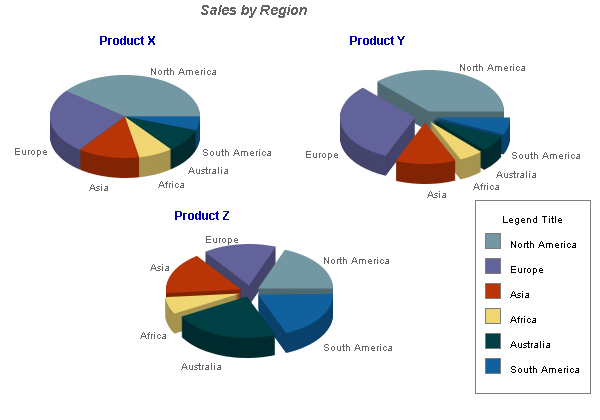
\includegraphics[width=.8\textwidth]{images/servlet3.png}
  \caption[A Pie chart]{Stolen from the net. Google for a pie chart...}
  \label{fig:pie}
\end{figure}

Many graphics packages can produce pdf files.
Embedded postscript (file extension .eps) are also a good candidate,
after converting them to pdf with the epstopdf tool. By the way: the
native format of Adobe Illustrator (ai) is similar enough to eps, so
that too can be processed with ps2pdf. Programs like {\em Visual
  Paradigm} are able to produce pdf files too. And sometimes open-office can
lend a helping hand, for by cutting and pasting Windows graphics into
a single page oodraw drawing, you can produce an very usable pdf file. 

Bitmap file types like png and jpeg take up a lot of space in your
final pdf document. 
Bitmap files take even more space if encoded into a pdf file.
If at all possible, stick to a vector format like eps or pdf (if
necessary derived from eps files). 

%\clearpage%to show headers

\section{A png example}
\label{page:pngexample}
If latex cannot fit the diagram on this page
(page~\pageref{page:pngexample}), 
 then you may find the diagram as figure~\vref{fig:pie}. And as you
 can see, you can easily reference pages and images.

%\clearpage%to show headers
\section{PDF from an UML package} 
\label{sec:pdffromuml}
% Note how this varioref expands to
% something like on the next page.
% and using a wrapfigure
\begin{wrapfigure}{r}{.4\textwidth}
  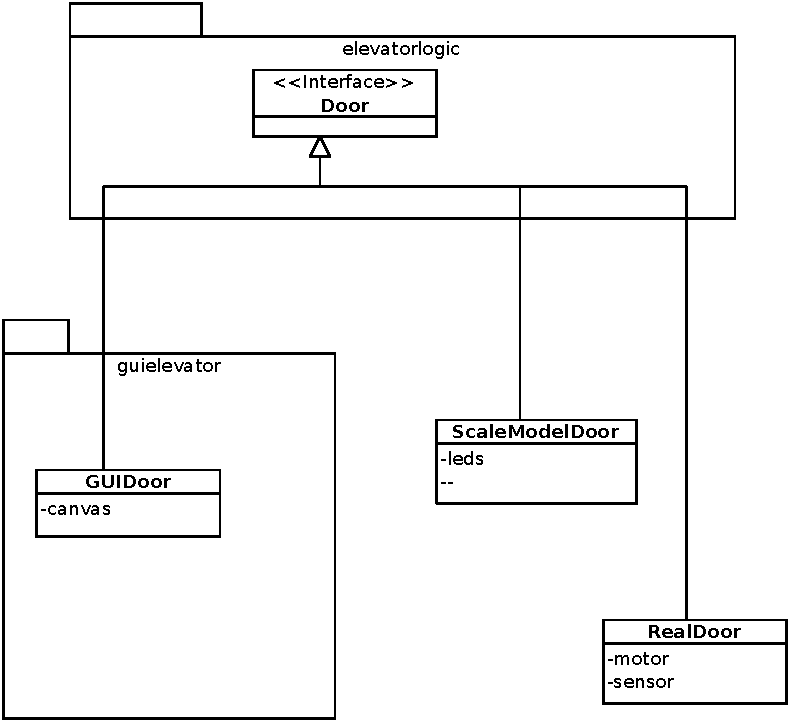
\includegraphics[width=.4\textwidth]{images/doorsystem.pdf}
  \caption{A class diagram made with Visual Paradigm}
  \label{fig:classdiagram}
\end{wrapfigure}
If the documentation you write is a design document of some software
package, you may want to include design diagrams.
No software engineering without a \define{\gls{UML}} diagrams\ldots.
You can see one generated with ``dia'', a vector drawing program that
understands the UML in figure~\ref{fig:classdiagram}
~\vpageref{fig:classdiagram}. This diagram is 'wrapped' in a \Code{wrapfigure} environment, so the text may flow around it

The diagram is not very sophisticated but shows an example of a vector
format file included via an eps$\rightarrow$ pdf conversion by
epstopdf.

Open source programs like umlet, but also commercial ones like Visual Pradigm are also able to produce
vector format graphics files. And sometimes it is helpful to add a box
that is a bit bigger then the picture you want to include.
This ensures that the so called bounding box does not cut of any lines
you want in your picture. Sometimes it is necessary to give these
tools a helping hand with inkscape, that is do a bit of tinkering to
get all details right. Or with \Code{pdfcrop} which typically comes with your \LaTeX installion.

\begin{figure}[htbp]
  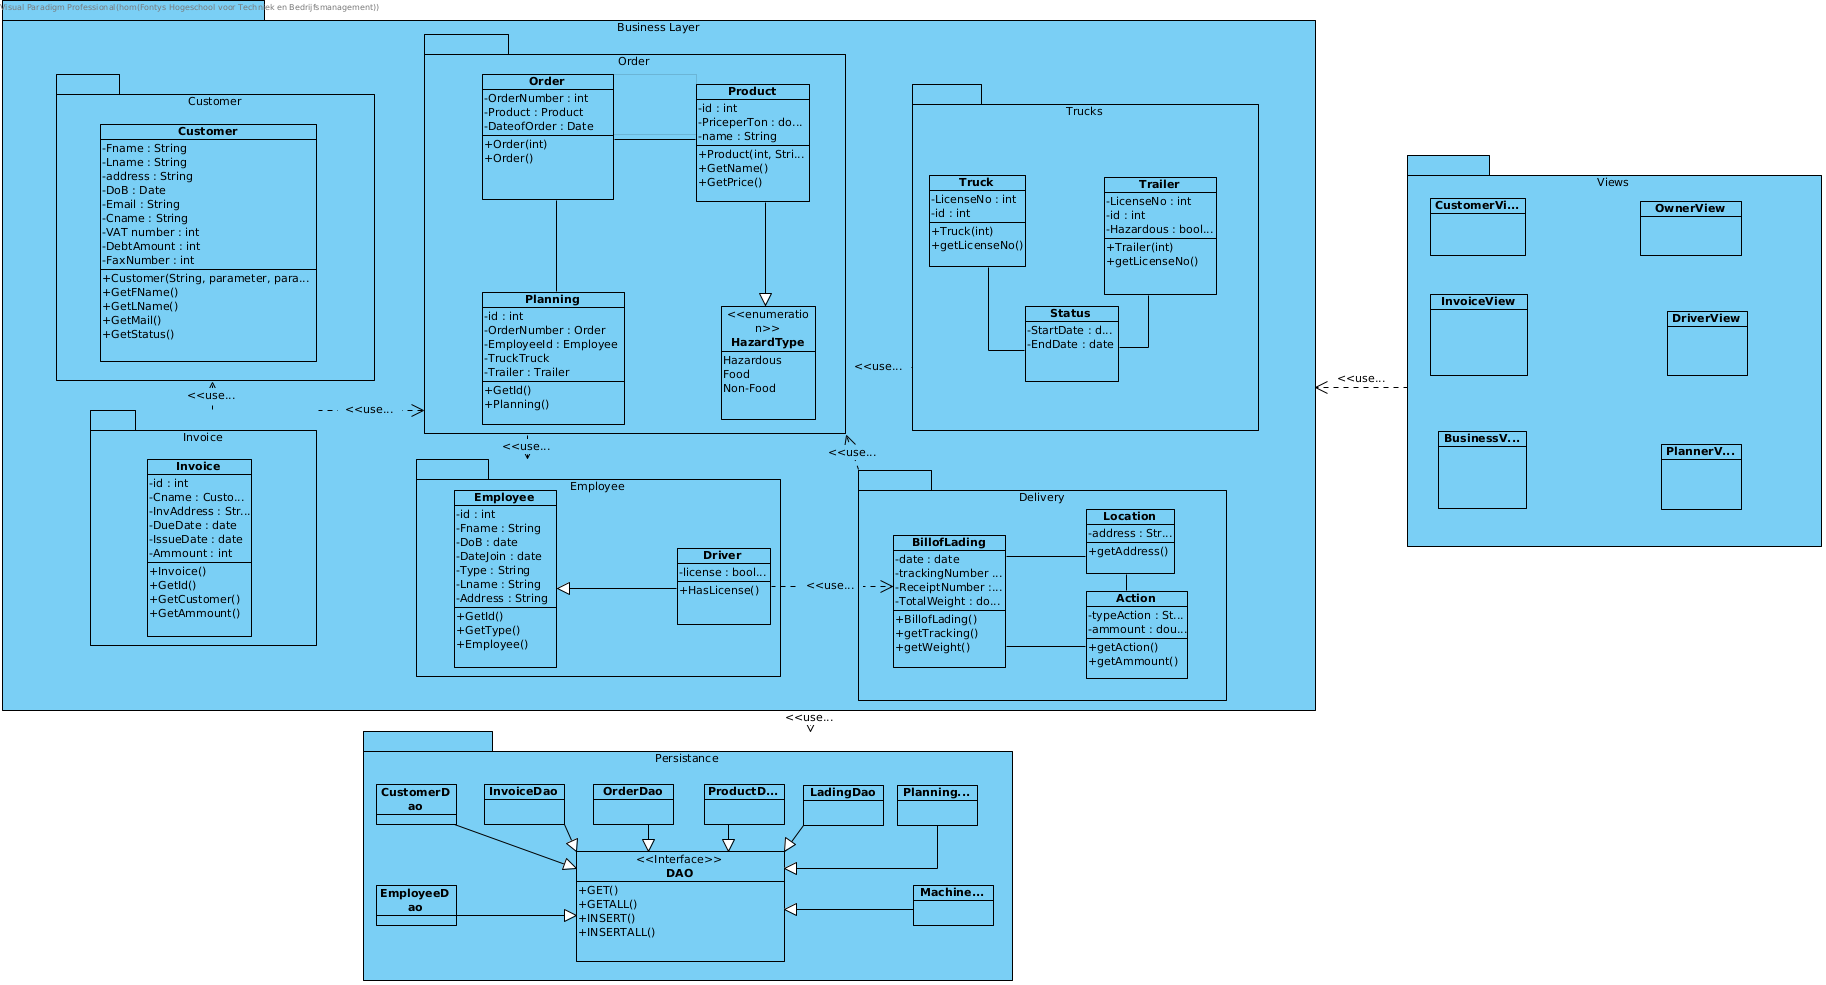
\includegraphics[width=\linewidth]{images/ClassDiagram1.png}
  \caption{You have been warned, NO PNG}
\end{figure}

The picture above is wrong on many fronts.
\begin{Itemize}
\item it uses png as image format, where a vector format is provided by the modeling application Visual Paradigm.
  However when you like a pixelated world such as in the game \gls{minecraft}, you might feel at home if you zoom in a bit.
\item The arrows point in all directions, which is bad style. A proper UML class diagram should be stylish to improve comprehensibility, as it is recognizable at a glance. Think of Da Vinci's Vitruvian man.
\item It has the VPP blues, that is the colours used are completely non-functional, and also impair readability because the used colour lowers the contract.
\end{Itemize}

Look on the next page how it is done properly.

% \begin{wrapfigure}{r}{.4\textwidth}
%   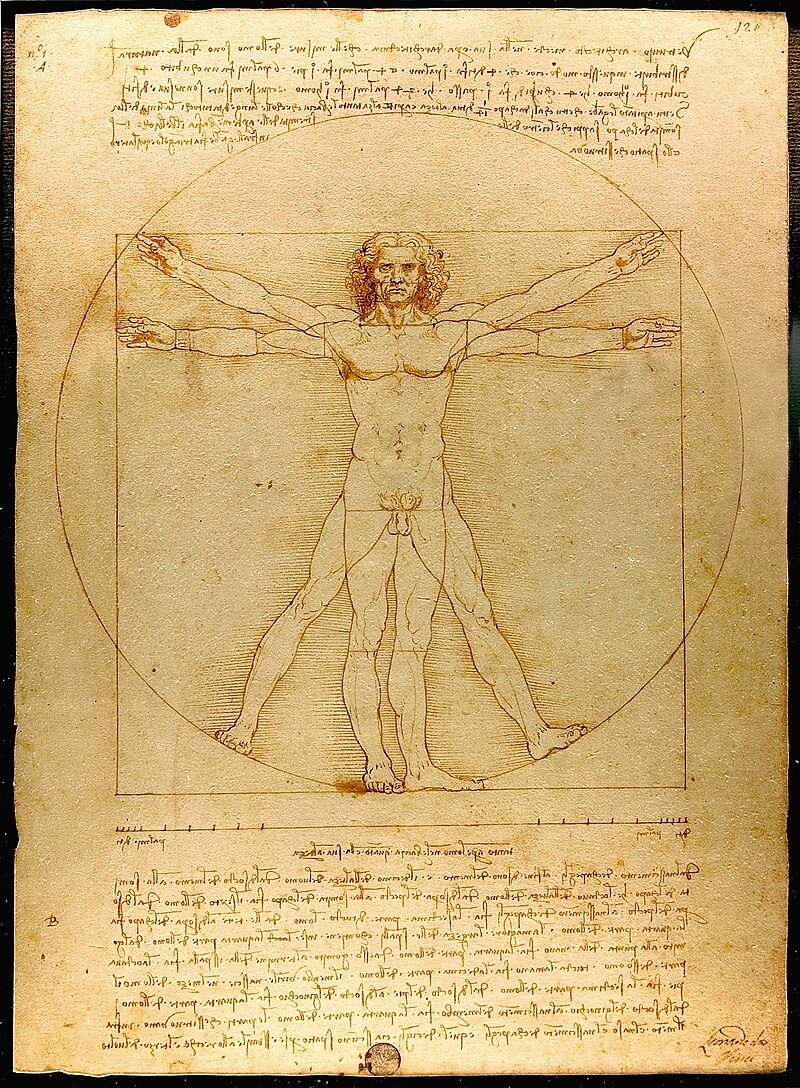
\includegraphics[width=.4\textwidth]{images/Da_Vinci_Vitruve_Luc_Viatour.jpg}
%   \caption{Left/right is has, up/down is inheritance (jpeg image)}
% \end{wrapfigure}
%\clearpage
\begin{figure}
  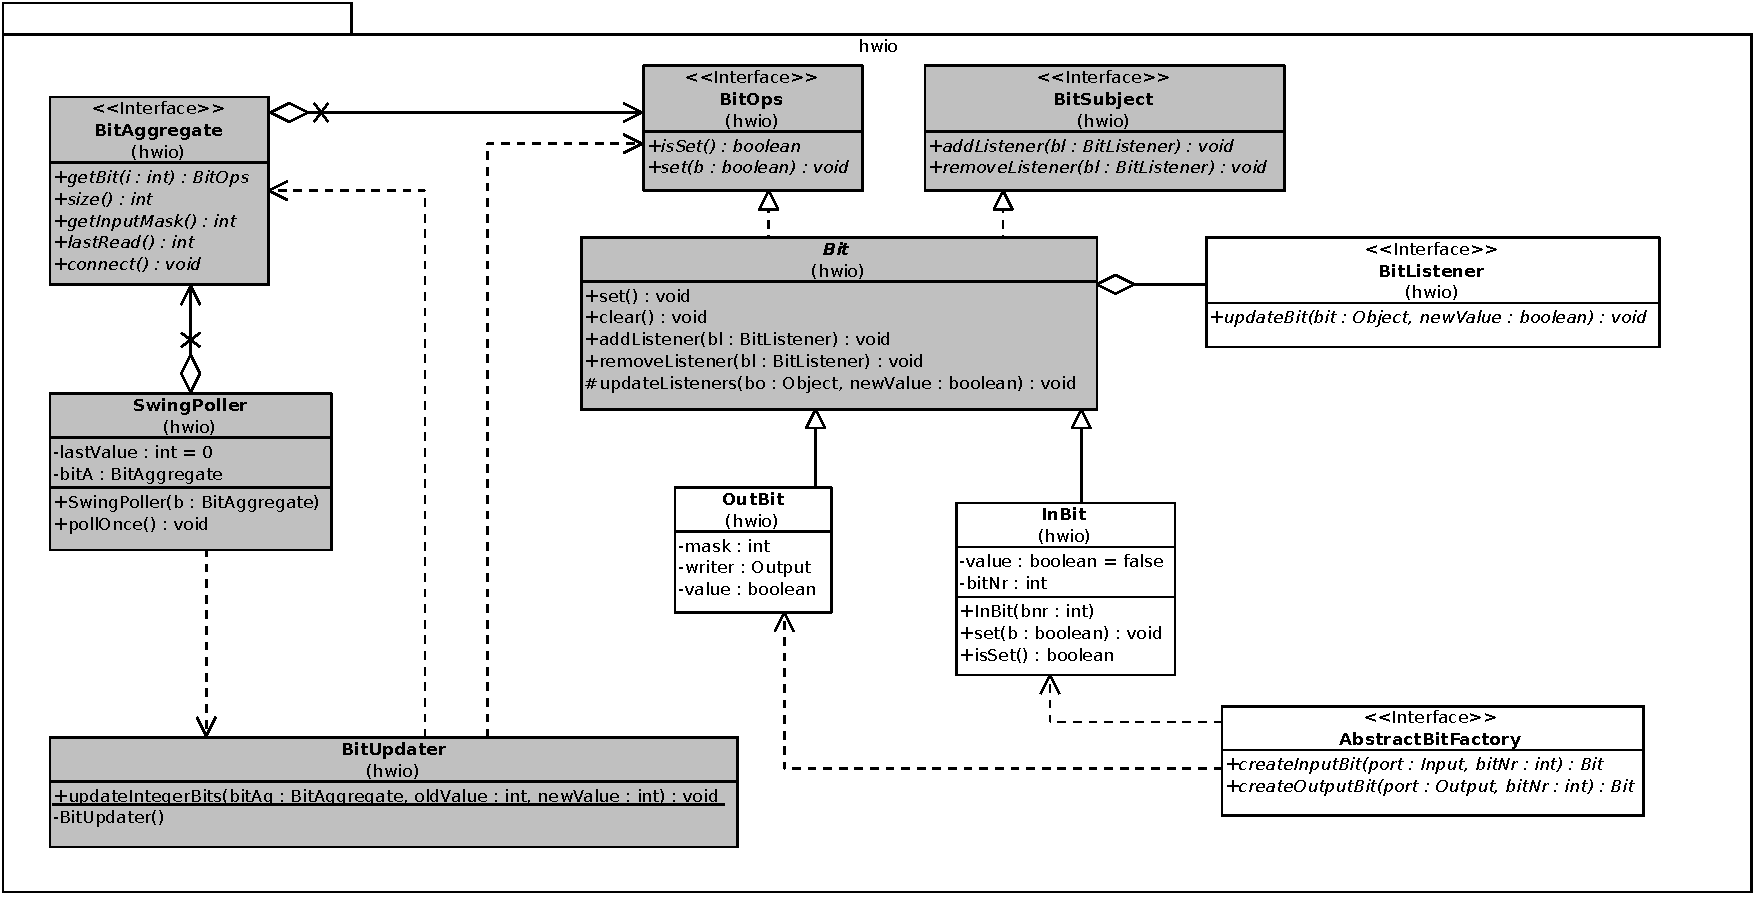
\includegraphics[width=\linewidth]{images/HWIO.pdf}
	\caption{UML made with Visual Paradigm, export to svg and then adapted with inkscape and end exported to pdf}
\end{figure}

\begin{figure}[htbp]
  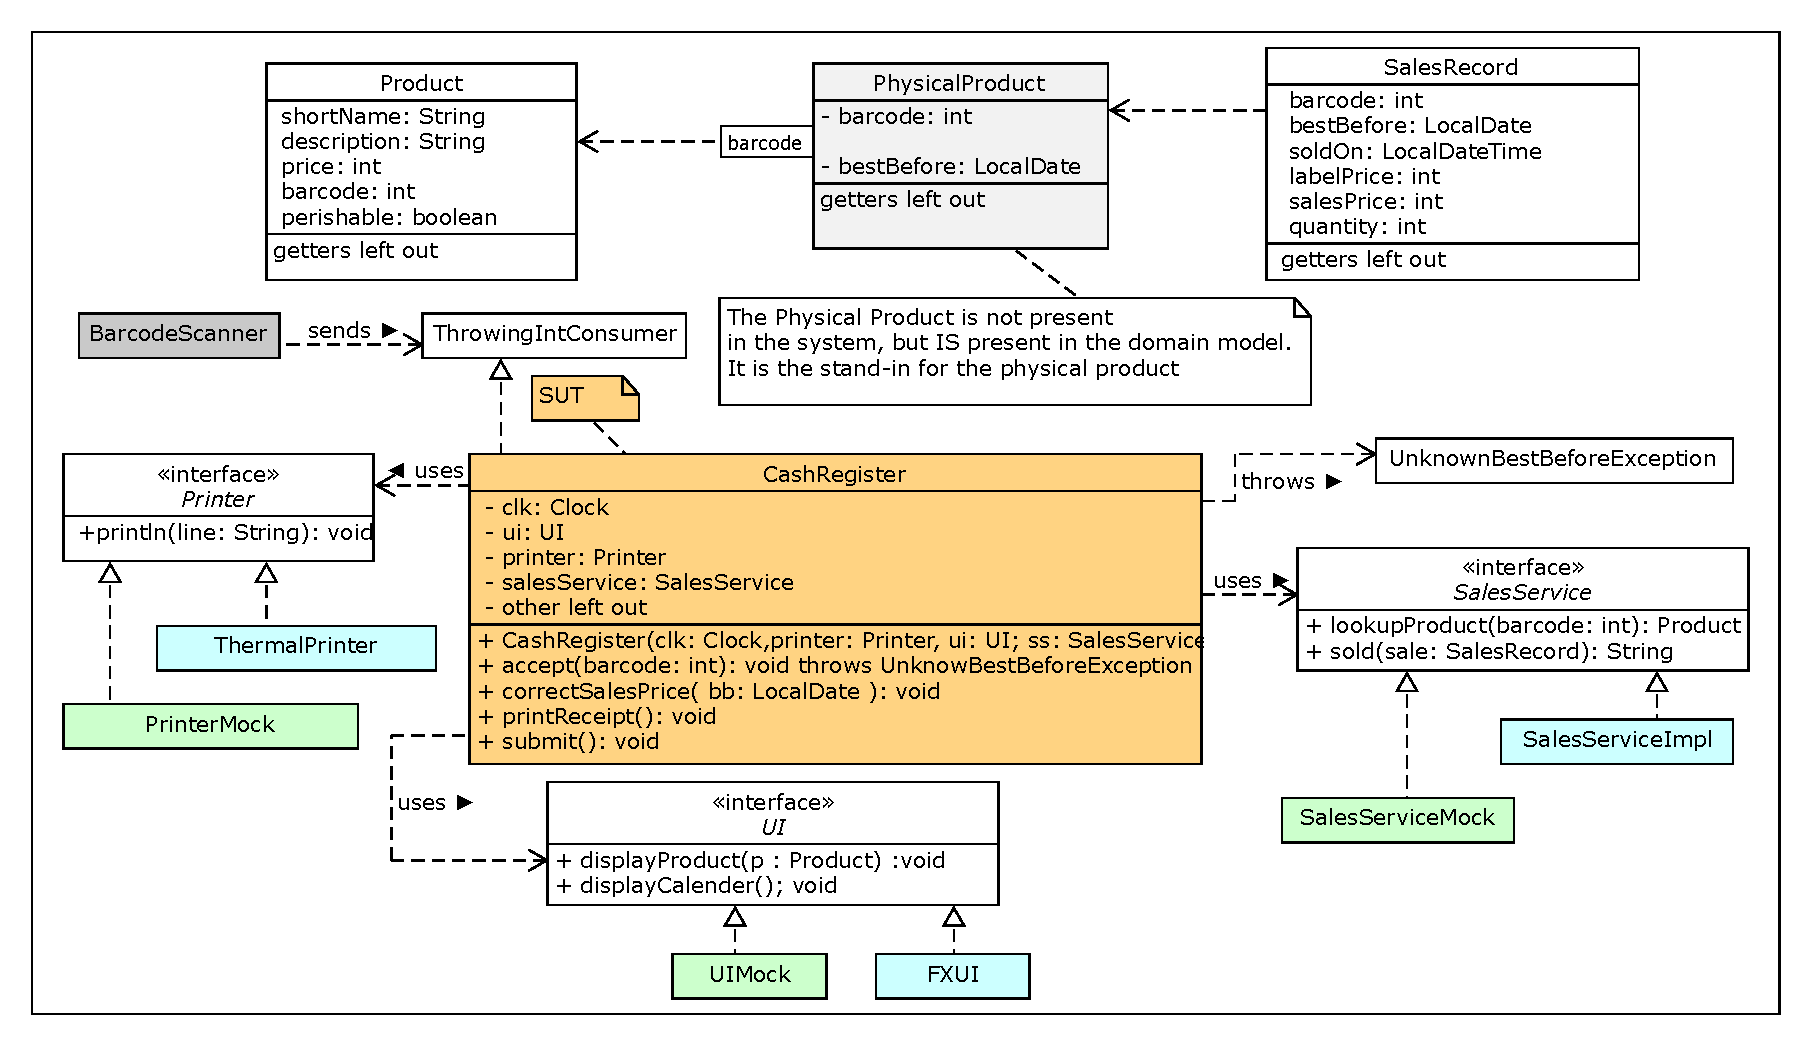
\includegraphics[width=\linewidth]{images/perishablesales.pdf}
  \caption{\label{fig:cashregistertest}Vector format (exported as pdf), with functional colour and a legend}
\end{figure}


\subsection{Stylish UML Class diagram}
\label{sec:stylish}
In the diagram of figure~\vref{fig:cashregistertest} above has style and uses functional colours which are simply explained in a legend.

Good style in a class diagram means:
\begin{Itemize}
\item There is always a direction. Arrows or triangles. They express dependencies.
\item Inheritance in the vertical direction only.
  \begin{Itemize}
    \item Any line that leaves at the top of a class box implies that this
      implements (dashed line) or extends (solid line), without looking where the line ends.
    \item Any triangle that enters at the bottom says that this class is extended or implemented for interfaces.
  \end{Itemize}
  \item All other relationships enter or leave at the left or right edge of the box, so you know things are used
  or this class is used/known.
  \begin{Itemize}
  \item If the local name is relevant, then that name is at the side of the using class, like barcode at the PhysicalProduct which identifies a Product in the system. Internally barcode is a simple number like an \Code{int} or \Code{long}.
  \end{Itemize}
\end{Itemize}

Other than style there are other advantages in this kind of diagrams.
\begin{Itemize}
\item You can zoom in as much as your viewer allows without getting a MineCraft world or worse.
\item A reviewer (the examiner, your coach or someone working with your documents) can select the texts in the diagram and can mark it. You too could do that to embellish the diagram.
\item There is no way that you can do that nicely with a pixel format like png or jpeg.
\end{Itemize}

%%% Local Variables: 
%%% mode: latex
%%% TeX-master: "main"
%%% End: 
